
\documentclass[a4paper, 12pt, oneside, BCOR1cm,toc=chapterentrywithdots,hidelinks]{scrbook}

\usepackage[a4paper]{geometry}
\usepackage{textcomp}
\usepackage{longtable}
%\usepackage{tabu}

\usepackage[ngerman, english]{babel}
\usepackage[utf8]{inputenc}
\usepackage{graphicx} 
\usepackage{acronym}
\usepackage{url}           	 
\usepackage{hyperref} 	
\usepackage{listings, color}	% for source code
\usepackage{scrlayer-scrpage}	% header and footer line
\usepackage{acronym}
\usepackage[ruled,vlined,algochapter]{algorithm2e}
\usepackage{tocbibind}
\usepackage{blindtext}
\usepackage{todonotes}


\usepackage{chngcntr}
\counterwithout{figure}{chapter}
\counterwithout{table}{chapter}
\counterwithout{algocf}{chapter} 
%\counterwithout{lstlisting}{chapter}
\AtBeginDocument{% the counter is defined later
  \counterwithout{lstlisting}{chapter}%
}
\renewcommand\lstlistingname{Code Fragment}

%for adding comments
\usepackage{verbatim}

% for tables
\usepackage{multirow}
\usepackage{xcolor}

% header and footer line - no header & footer line on pages where a new chapter starts
\pagestyle{scrheadings}


\begin{document}

\frontmatter
%Titlepage
\thispagestyle{empty}
\begin{center}

%\resizebox{1\textwidth}{!}{%
%
\includegraphics[height=3 pt]{img/tu-logo.png}%
%\quad
%
\includegraphics[height=2 pt]{img/DAI-Labor.png}%
%}

\begin{figure}[t]
    \centering
    
\includegraphics[width=4cm]{./img/tu-logo.png}%
%    \qquad
%    \includegraphics[width=3.3cm]{dima_logo.png}%
\end{figure}


{\LARGE \textbf{Technische Universit\"at Berlin}}

\vspace{0.3cm}

{\normalsize 
%Faculty IV - Electrical Engineering and Computer Science \\ 
Chair of Agent Technologies in Business Applications and Telecommunications\\[1.6mm]}

\vspace{2.0cm}

{\LARGE Master's Thesis}\\

\vspace{2.5cm}
\Large \textbf{Reinforcement Learning based \\ Strategic Bidding for a Virtual Power Plant \\ in the Frequency Containment Reserve Market}

\vspace{1.0cm}

\normalsize{
Jan-Lukas Simon Valentin Pflaum \\
Degree Program: Information Systems Management\\
Matriculation Number: 407059\\

\vspace*{1.7cm}
\textbf{Reviewers}\\
Prof. Dr. Dr. h.c. Sahin Albayrak\\
Prof. Dr. habil. Odej Kao\\
\vspace*{0.5cm}
\textbf{Advisor}\\
M.Sc Izgh Hadachi\\
\vspace{0.5 cm}

\textbf{Submission Date}\\
14.12.2022\\
}
\end{center}


\thispagestyle{empty}
\cleardoublepage
    
%Self-assertion
\newpage

\thispagestyle{empty}

\begin{large}

\vspace*{6cm}

\noindent
Hereby I declare that I wrote this thesis myself with the help of no more than the mentioned literature and auxiliary means.
\vspace{2cm}

\noindent
Berlin, DD.MM.YYYY

\vspace{3cm}

\hspace*{7cm}%
\dotfill\\
\hspace*{8.2cm}%
\textit{Firstname, Lastname(s)}

\end{large}
 
\thispagestyle{empty}
\cleardoublepage

% Abstract in Deutsch
\addchap*{Zusammenfassung}
Tipps zum Schreiben dieses Abschnitts finden Sie unter \cite{wallwork_177}

% Abstract
\addchap*{Abstract}
%\thispagestyle{empty}   - 
%For tips on writing this section, refer \cite{wallwork_177} 
The abstract should be 1-2 paragraphs. It should include:
\begin{itemize}
 \item a statement about the problem that was addressed in the thesis,
 \item a specification of the solution approach taken,
 \item a summary of the key findings. 
\end{itemize}

For additional recommendations see \cite{wallwork_177}. 

\noindent
%This template is intended to give an introduction of how to write diploma and master thesis at the chair 'Architektur der Vermittlungsknoten' of the Technische Universit�t Berlin. Please don't use the term 'Technical University' in your thesis because this is a proper name. 
%\\
%\\
%On the one hand this PDF should give a guidance to people who will soon start to write their thesis. The overall structure is explained by examples. On the other hand this text is provided as a collection of LaTeX files that can be used as a template for a new thesis. Feel free to edit the design.
%\\
%\\
%It is highly recommended to write your thesis with LaTeX. I prefer to use Miktex in combination with TeXnicCenter (both freeware) but you can use any other LaTeX software as well. For managing the references I use the open-source tool jabref. For diagrams and graphs I tend to use MS Visio with PDF plugin. Images look much better when saved as vector images. For logos and 'external' images use JPG or PNG. In your thesis you should try to explain as much as possible with the help of images.
%\\
%\\
%The abstract is the most important part of your thesis. Take your time to write it as good as possible. Abstract should have no more than one page. It is normal to rewrite the abstract again and again, so  probaly you won't write the final abstract before the last week of due-date. Before submitting your thesis you should give at least the abstract, the introduction and the conclusion to a native english speaker. It is likely that almost no one will read your thesis as a whole but most people will read the abstract, the introduction and the conclusion.
%\\
%\\
%Start with some introductionary lines, followed by some words why your topic is relevant and why your solution is needed concluding with 'what I have done'. Don't use too many buzzwords. The abstract may also be read by people who are not familiar with your topic.
  
% Acknowledgments  
\addchap*{Acknowledgments}
For recommendations on writing your Acknowledgments see \cite{wallwork_306}.

%table of contents
\addtocontents{toc}{\protect\setcounter{tocdepth}{-1}}
\tableofcontents
\addtocontents{toc}{\protect\setcounter{tocdepth}{3}}

%footnote
\newcommand\blfootnote[1]{%
  \begingroup
  \renewcommand\thefootnote{}\footnote{#1}%
  \addtocounter{footnote}{-1}%
  \endgroup
}


%list of figures
\listoffigures

%list of tables
\listoftables



    

    

% List of Abbreviations
\onecolumn
\addchap{List of Abbreviations}
\begin{acronym}[Bash]   
 \acro{DAI Labor}{Distributed Artificial Intelligence Laboratory}
\end{acronym}
\onecolumn


%algorithms
\listofalgorithms
\addcontentsline{toc}{chapter}{List of Algorithms}

%In case, code fragments have to be added
%\renewcommand{\lstlistlistingname}{List of Code Fragments}
%\lstlistoflistings
%\addcontentsline{toc}{chapter}{List of Code Fragments}

\mainmatter % comment single chapters for faster compilation
    \chapter{Introduction\label{cha:intro}}

... should include the following:
\begin{itemize}
\item motivation (why is this problem interesting? offer examples),
\item research challenge (what is the obstacle to be overcome?),
\item novelty (was this problem already solved?),
\item anticipated impact (how does solving this problem impact our world?).
\end{itemize}

This chapter should include the following sections.

\section{Motivation\label{sec:moti}}
This section should 
\begin{itemize}
    \item answer the question - why is this problem interesting? 
    \item offer examples illustrating the problem.
\end{itemize}


\section{Research Challenge\label{sec:objective}}
This section should answer the question -
\begin{itemize}
    \item what is the obstacle to be overcome?
\end{itemize}

\section{Novelty \label{sec:scope}}
This section should answer the question -
\begin{itemize}
    \item was this problem already solved?
\end{itemize}

\section{Anticipated Impact \label{sec:outline}}
This section should answer the question -
\begin{itemize}
    \item how does solving this problem impact our world?
\end{itemize}

Conclude this subsection with an image describing 'the big picture'. How does your solution fit into a larger environment? You may also add another image with the overall structure of your component.

'Figure \ref{fig:intro} shows Component X as part of ...' 
\\


 The 'structure' or 'outline' section gives a brief introduction into the main chapters of your work. Write 2-5 lines about each chapter. Usually diploma thesis are separated into 6-8 main chapters. 
 \\
 \\
 \noindent This example thesis is separated into 7 chapters.
 \\
 \\
 
% 1. Introduction (3 pages)
% 2. Research Problem (???)
% 3. SOTA
% 4. Requirements (5-10 pages)
% 4. Concept (12-18 pages)
% 5. Implementation (9-12 pages)
% 6. Experiment and Analytical Evaluation (6-9 pages)
% 7. Conclusion and Outlook (4-6 pages)

 
 \textbf{Chapter \ref{cha:chapter2}} is usually termed 'Related Work', 'State of the Art' or 'Fundamentals'. Here you will describe relevant technologies and standards related to your topic. What did other scientists propose regarding your topic? This chapter makes about 20-30 percent of the complete thesis.
 \\
 \\
 \textbf{Chapter \ref{cha:chapter3}} analyzes the requirements for your component. This chapter will have 5-10 pages.
 \\
 \\
 \textbf{Chapter \ref{cha:chapter4}} is usually termed 'Concept', 'Design' or 'Model'. Here you describe your approach, give a high-level description to the architectural structure and to the single components that your solution consists of. Use structured images and UML diagrams for explanation. This chapter will have a volume of 20-30 percent of your thesis.
 \\
 \\
 \textbf{Chapter \ref{cha:chapter5}} describes the implementation part of your work. Don't explain every code detail but emphasize important aspects of your implementation. This chapter will have a volume of 15-20 percent of your thesis.
 \\
 \\
 \textbf{Chapter \ref{cha:chapter6}} is usually termed 'Evaluation' or 'Validation'. How did you test it? In which environment? How does it scale? Measurements, tests, screenshots. This chapter will have a volume of 10-15 percent of your thesis.
 \\
 \\
 \textbf{Chapter \ref{cha:chapter7}} summarizes the thesis, describes the problems that occurred and gives an outlook about future work. Should have about 4-6 pages.
    \chapter{Scientific Background\label{cha:chapter2}}
... should include the following:
\begin{itemize}
    \item definitions / technical terms,
    \item theoretical foundations / principles,
    \item descriptions of algorithms, hardware, software, and/or systems employed.
\end{itemize}



\begin{figure}[h]
\centering
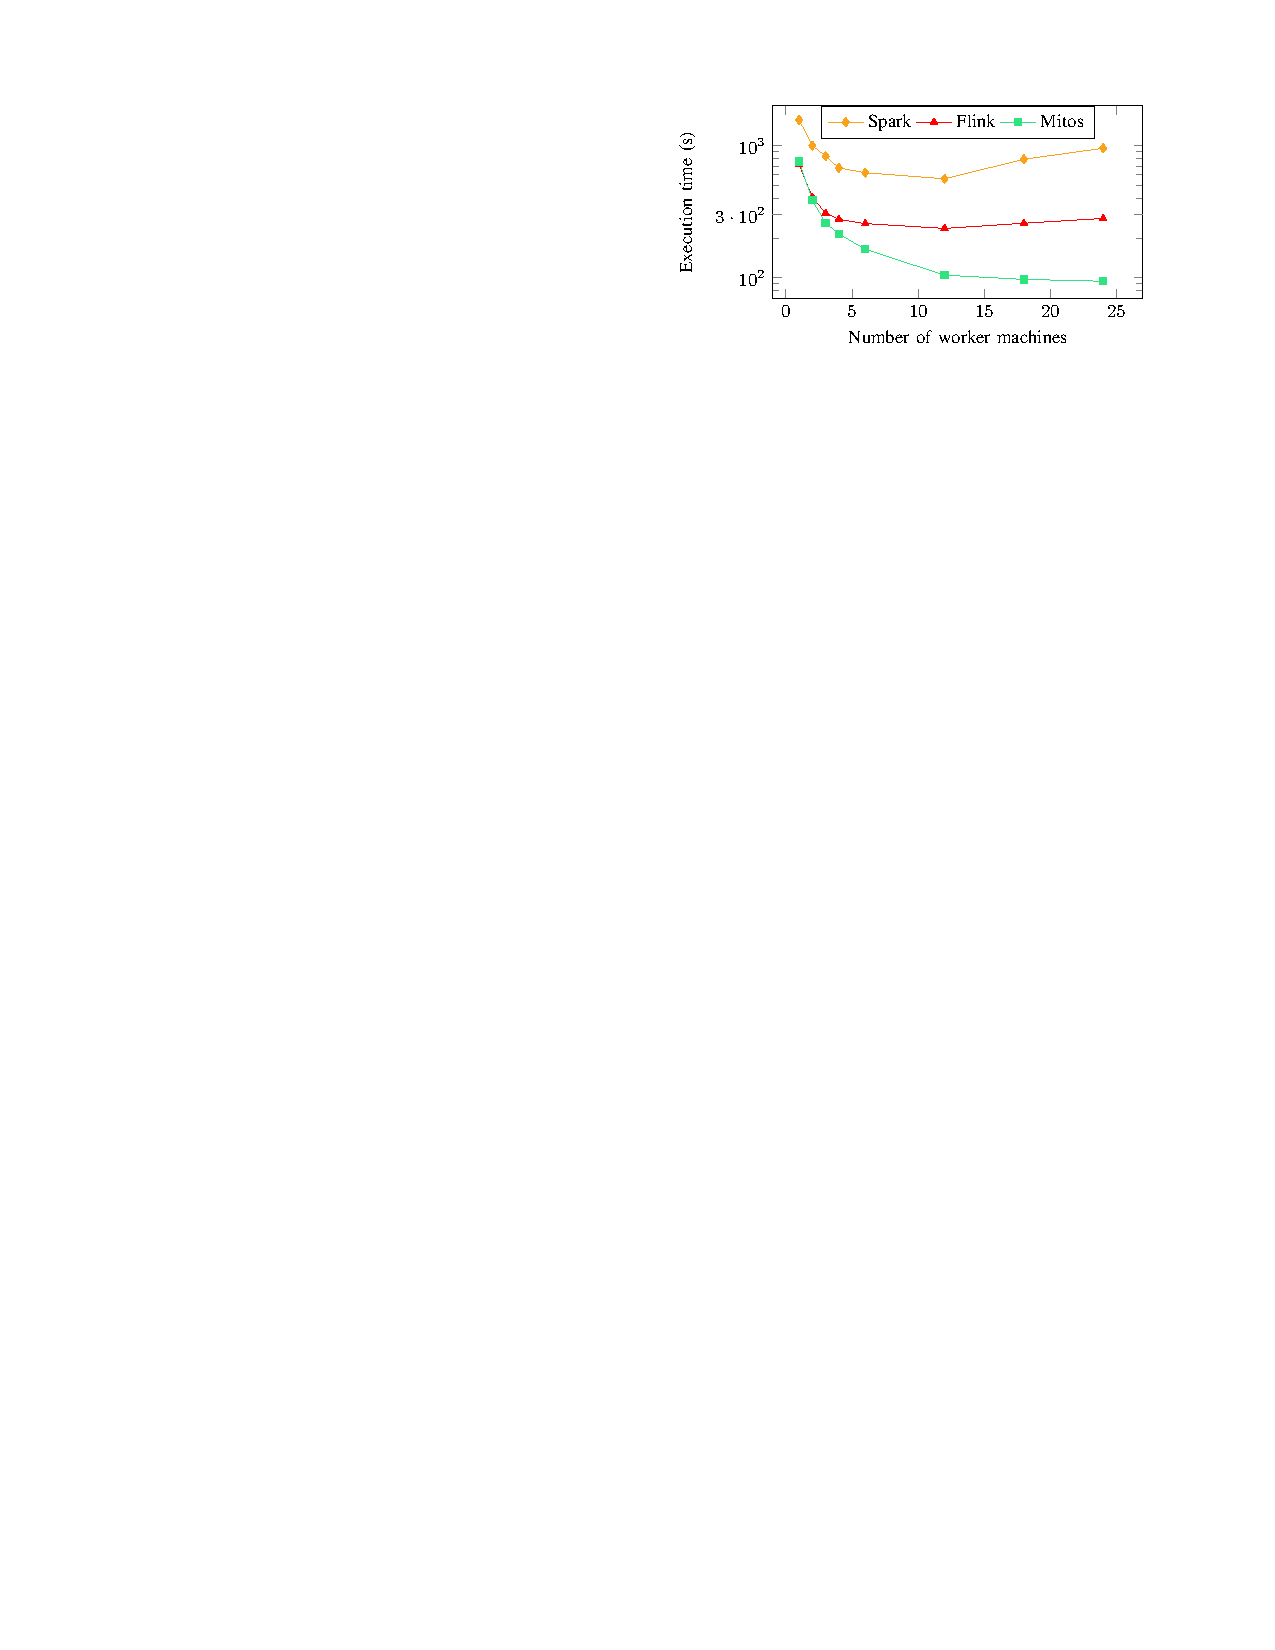
\includegraphics[width=0.6\textwidth]{./img/strong_scaling.pdf}
\caption{Strong scaling for Visit Count\cite{GevayRBMQM21}.}
\end{figure}

Suggestion: Figures could be inserted in pdf form to avoid pixelation when the image is magnified.

This section is intended to give an introduction about relevant terms, technologies and standards in the field of X. You do not have to explain common technologies such as HTML or XML. 



    \chapter{Research Problem \label{sec:problem}}

... should include the following:
\begin{itemize}

\item a succinct, precise, and unambiguous statement of the research problem or question to be solved,
\item goals and subproblems that will be explored, including the scope of the thesis (i.e., what is in and out of scope).
\end{itemize}
\begin{comment} 
\begin{table}[h!]
\begin{center}
\begin{tabular}{ |c|c|c| } 
 \hline
 Column1 & Column2 & Column3 \\ [0.5ex] 
 \hline
 cell1 & cell2 & cell3 \\ 
 cell4 & cell5 & cell6 \\ 
 cell7 & cell8 & cell9 \\ 
 \hline
\end{tabular}
\caption{An Example Table.}
%\label{table:1}
\end{center}
\end{table}
\end{comment} 


\begin{table}[ht]
\begin{center}
\footnotesize{
\begin{tabular}{ c|c } 
 \hline
  Area (Million sq. miles) & Calling Code \\
  \hline
 0.29 & 56\\
 0.3 & 90\\
 3.8 & 1\\
 0.5 & 51\\
% \rowfont{\color{red}}
\textcolor{red}{600} & \textcolor{red}{9800}\\
 \hline
 \multicolumn{1}{c}{Pearson = 1.0} & \multicolumn{1}{c}{Spearman’s = 0.1}
\end{tabular}
}
\caption{Correlation in the existence of outlier\cite{EsmailoghliQZ21}.}
%\label{table:1}
\end{center}
\end{table}


    \input{./chapters/03_State_of_the_art.tex}
    \chapter{Requirements\label{cha:requirements}}

    \chapter{Solution}

... should include the following:
\begin{itemize}
\item research methodology (e.g., prototype and experiments, case study, literature survey, theoretical analysis),
\item derivations and descriptions of algorithms, hardware, software, and/or systems developed.
\end{itemize}
\begin{comment} 
\begin{algorithm}
\SetAlgoLined
\KwResult{Write here the result }
 initialization\;
 \While{While condition}{
  instructions\;
  \eIf{condition}{
    instructions1\;
    instructions2\;
    }{
    instructions3\;
    }
    }
 \caption{An Example Algorithm}
 %\label{alg:algorithm1}
\end{algorithm}
\end{comment} 


\begin{algorithm}
\SetAlgoLined
\SetKwInOut{Parameter}{Parameters}
\Parameter{\\e : Tuple to be inserted.\\
te (e) : Event-time of e. }
 S ← slice that covers te (e);\\
  \eIf{S starts at te (e)}{
    //Slice before S must be fixed.\\
    change the type of the slice before S to combined;\\
    add e to S;\\
    }{
    // S does not start at te (e).\\
    change tend (S) to te (e) (excluding te (e) from S);\\
 change type of S to flexible;\\
add slice in [te (e), former tend (S)] with former type of S.\\
add e to the new slice.\\
    }
 \caption{Splitting a Session\cite{TraubGCBKRM20}.}
 %\label{alg:algorithm1}
\end{algorithm}
    \chapter{Concept\label{cha:concept}}

    \chapter{Implementation}

... should include the following:
\begin{itemize}
\item research methodology (e.g., prototype and experiments, case study, literature survey, theoretical analysis),
\item derivations and descriptions of algorithms, hardware, software, and/or systems developed.
\end{itemize}
\begin{comment} 
\begin{algorithm}
\SetAlgoLined
\KwResult{Write here the result }
 initialization\;
 \While{While condition}{
  instructions\;
  \eIf{condition}{
    instructions1\;
    instructions2\;
    }{
    instructions3\;
    }
    }
 \caption{An Example Algorithm}
 %\label{alg:algorithm1}
\end{algorithm}
\end{comment} 


\begin{algorithm}
\SetAlgoLined
\SetKwInOut{Parameter}{Parameters}
\Parameter{\\e : Tuple to be inserted.\\
te (e) : Event-time of e. }
 S ← slice that covers te (e);\\
  \eIf{S starts at te (e)}{
    //Slice before S must be fixed.\\
    change the type of the slice before S to combined;\\
    add e to S;\\
    }{
    // S does not start at te (e).\\
    change tend (S) to te (e) (excluding te (e) from S);\\
 change type of S to flexible;\\
add slice in [te (e), former tend (S)] with former type of S.\\
add e to the new slice.\\
    }
 \caption{Splitting a Session\cite{TraubGCBKRM20}.}
 %\label{alg:algorithm1}
\end{algorithm}
    \chapter{Experimental and Analytical Evaluation\label{cha:chapter4}}

\section{Experimental Setup\label{sec:exp}}
... should include the following:
\begin{itemize}

\item define experimental data and workload(s),
\item discussion about the selection and interpretation of the evaluation metrics,
\item discussion about the computing environment, including hardware, software, tools.
\end{itemize}

\begingroup
\renewcommand\thesection{5.X}


\section{Design and an Interpretation of the Results (For each Experiment Class X)}
... should include the following:
\begin{itemize}
\item which experiments will be conducted and why?
\item for each experiment, what are objectives, baselines, and expected results?
\item description and an interpretation of the experimental results,
\item explanation for any anomalies or any unexpected behavior.
\end{itemize}
\endgroup
\begin{comment} 
\section{For each Experiment Class X}

\subsection{Experimental Design}
This sub-section should answer the questions -
\begin{itemize}
\item which experiments will be conducted and why?
\item for each experiment, what are objectives, baselines, and expected results?
\end{itemize}


\subsection{Interpretation of the Results}
This sub-section should include
\begin{itemize}
\item 	description and an interpretation of the experimental results.
\item 	explanation for any anomalies or any unexpected behavior.
\end{itemize}
\end{comment} 


    \chapter{Conclusion and Outlook\label{cha:conclusion}}
... should include the following:
\begin{itemize}

\item problem restated and a brief summary of the methodology,
\item student contributions (e.g., survey, open-source software, journal publication),
\item a brief summary of the findings and results,
\item limitations and generalizability of the findings and results.
\item lessons learned,
\item recommendations for future research.

\end{itemize}



% ---------------------------------------------------------------

%Bibliography
\begingroup
\raggedright
\bibliographystyle{splncs03}
%\bibliographystyle{acm}
\bibliography{bibliography}
\endgroup

%appendix
\addchap{Appendix A. Further Details on the Solution Approach}

\addchap{Appendix B. Extended Version of the Experimental Results}


\end{document}
